\chapter{Finite Fields and Sequential Arithmetic Circuits}
\label{ch:prelim_GF}
This chapter provides a mathematical background for understanding 
finite fields (Galois fields) and explains how to design Galois field (GF) arithmetic circuits.
We first introduce the mathematical concepts of groups, rings, fields, and 
polynomials. 
We then apply these concepts to create Galois field arithmetic functions and 
explain how to map them to a Boolean circuit implementation.
Additionally, we introduce a special type of sequential arithmetic hardware based on normal basis, as well
as the normal basis theory behind the designing such hardware.

The material is referred from \cite{galois_field:mceliece, ftheory:2006, ff:1997} for Galois field concepts, 
\cite{mastro:1989, PT:1985, acar:1998, wu:2002, Knezevic:2008} for hardware design over Galois fields 
and previous work by Lv \cite{lv:phd}.
Normal basis theory in this section is referred from \cite{normal_book, gao:phd_normal_basis} and sequential
normal basis arithmetic hardware designs come from \cite{mullinONB,MasseyOmura,agnew1991implementation, RHmulti}.

\section{Commutative Algebra}
\label{sec:algebra}
\subsection{Group, Ring and Field}
\begin{Definition}
An {\bf Abelian group} is a set $\mathbb{S}$ with a binary operation $'+'$
which satisfies the following properties: 
\begin{itemize}
\item {\it Closure Law:} For every $a, b \in \mathbb{S}, a + b \in \mathbb{S}$  
\item {\it Associative Law:} For every $a, b, c \in \mathbb{S}, (a + b) + c = a + (b + c)$
\item {\it Commutativity:} For every $a, b \in \mathbb{S}, a + b = b + a$. 
\item {\it Additive Identity:} There is an identity element $0 \in \mathbb{S}$
such that for all $a \in \mathbb{S};$ $a + 0 = a$.
\item {\it Additive Inverse:} If $a \in \mathbb{S}$, then there is an
element $a^{-1} \in \mathbb{S}$ such that $ a + a^{-1} = 0$.
\end{itemize}
\end{Definition}

The set of integers $\mathbb{Z}$ forms an Abelian group under the addition operation. 

\begin{Definition}
Given a set $\mathbb{R}$ with two binary operations, $'+'$ and $'\cdot'$, 
and element $0 \in \mathbb{R}$, the system $\mathbb{R}$ is called a {\bf commutative ring with unity} if the following properties hold:
\begin{itemize}
\item $\mathbb{R}$ forms an Abelian group under the '+' operation with additive identity element $0$.
\item {\it Multiplicative Distributive Law}: For all $a, b, c \in$ $\mathbb{R}$, $a\cdot (b + c) = a\cdot b + a\cdot c$.
\item {\it Multiplicative Associative Law}: For every $a, b, c\in \mathbb{R}$, $a\cdot (b\cdot c) = (a\cdot b)\cdot c$. 
\item {\it Multiplicative Commutative Law}: For every $a,b \in \mathbb{R}$, $a\cdot b = b\cdot a$
\item {\it Identity Element}: There exists an element $1 \in$ $\mathbb{R}$ 
such that for all $a \in \mathbb{R}$, $a\cdot 1 = a =1\cdot a$
\end{itemize}
\end{Definition}

{\bf Ring} is a broad algebraic concept. In this dissertation, this word is used to refer a special 
sort of ring -- {\bf commutative ring with unity}. Two common 
examples of such rings are the set of integers, $\mathbb{Z}$, and the set of 
rational numbers, $\mathbb{Q}$. While both of these examples are
rings with an infinite number of elements, the number of elements in a ring 
can also be finite, such as the ring of integers modulo $n$ ($\Z_n$).

\begin{Definition}
A {\bf field} $\mathbb{F}$ is a commutative ring with unity, where every
non-zero element in $\mathbb{F}$ has a multiplicative inverse; {\it i.e.} $\forall
a \in \mathbb{F} - \{0\}$, $\exists \hat{a} \in \mathbb{F}$ such that $ a \cdot
\hat{a} = 1$.
\end{Definition}

A field is defined as a ring with one extra condition: the presence of a 
multiplicative inverse for all non-zero elements.
Therefore, a field must be a ring while a ring is not necessarily a field.
For example, the set $\mathbb{Z}_{2^k} = \{0,1,\cdots, 2^k-1\}$ forms a finite ring.
However, $\mathbb{Z}_{2^k}$ is not a field because not every element in
$\mathbb{Z}_{2^k}$ has a multiplicative inverse. 
In the ring $\mathbb{Z}_{2^3}$, for 
instance, the element $5$ has an inverse ($5\cdot5\pmod{8}=1$) but the element $4$
does not.

An important concept in field theory is {\bf field extension}. The idea behind a
field extension is to take a base field and construct a larger field which 
contains the base field as well as satisfies additional properties. For example,
the set of real numbers $\mathbb{R}$ forms a field; one extension of 
$\mathbb{R}$ is the set of complex numbers $\mathbb{C}=\mathbb{R}(i)$. Every
element of $\mathbb{C}$ can be represented as $a+b\cdot i$ where $a,b \in \mathbb{R}$,
hence $\mathbb{C}$ is a two-dimensional extension of $\mathbb{R}$.

Like rings, fields can also contain either an infinite or a finite number of 
elements. 
In this dissertation we focus on finite fields -- also known as Galois fields, 
the construction of their field extensions, and their applications on circuit verification and abstraction techniques.

\subsection{Finite Field}
Finite fields find widespread applications in 
many areas of electrical engineering and computer science such as error-
correcting codes, elliptic curve cryptography, digital signal processing, 
testing of VLSI circuits, among others.
In this dissertation, we specifically focus on their application to 
the FSM traversal of sequential Galois field circuits as well as abstraction refinement based on UNSAT core extraction.
This section describes the relevant Galois field concepts
\cite{galois_field:mceliece} \cite{ftheory:2006} \cite{ff:1997}
and hardware arithmetic designs over such fields \cite{mastro:1989} \cite{PT:1985} 
\cite{acar:1998} \cite{wu:2002} \cite{Knezevic:2008}. 

%%%%%%%%%%%%%%%%%%%%%%%%%%%%%%%%%%%%%%%%%%%%%%%%%%%%%%%%%%%%%%%%%%%%%%%%%%%%

\begin{Definition} 
A {\bf Galois field}, denote $\Fq$, is a field with a finite
number of elements, $q$. The number of elements $q$ of the field is
a power of a prime integer, {\it i.e.} $q = p^k$, where $p$ is a prime
integer, and $k \geq 1$. Thus a Galois field can also be denoted as 
$\F_{p^{k}}$.
\end{Definition}

Fields of the form $\F_{p^{k}}$ are called Galois extension fields.
We are specifically interested in extension fields of type 
$\Fkk$, where $k > 1$. These are extensions of the binary
field $\F_2$.

\begin{table}[!h]
\caption{Addition and multiplication operations over $\F_2$.}
	\centering
	\begin{tabular}{m{1cm}|l|ll|m{1cm}}
	\hhline{~---~}
	\multirow{3}{*}{} & $+$ & $0$ & $1$ & \multirow{3}{*}{} \\
	\hhline{~---~}
	& $0$ & $0$ & $1$ & \\
	& $1$ & $1$ & $0$ & \\
	\hhline{~---~}
	\multicolumn{5}{c}{}\\
	\multicolumn{5}{c}{Addition over $\F_2$}\\
	\end{tabular}
	\quad
	\begin{tabular}{m{1cm}|l|ll|m{1cm}}
	\hhline{~---~}
	\multirow{3}{*}{} & $\cdot$ & $0$ & $1$ & \multirow{3}{*}{} \\
	\hhline{~---~}
	& $0$ & $0$ & $0$ & \\
	& $1$ & $0$ & $1$ & \\
	\hhline{~---~}
	\multicolumn{5}{c}{}\\
	\multicolumn{5}{c}{Multiplication over $\F_2$}\\
	\end{tabular}
\end{table}

Notice that addition over $\F_2$ is a Boolean {\sc XOR} operation, 
because it is performed modulo $2$.
Similarly, multiplication over $\F_2$ performs a Boolean {\sc AND} operation.


Algebraic extensions of the binary field $\F_{2}$  
are generally termed as {\it binary extension fields} $\Fkk$.
Where elements in $\F_2$ can only represent $1$ bit, elements in $\Fkk$ 
represent a $k$-bit vector.
This allows them to be widely used in digital hardware applications.
In order to construct a Galois field of the form $\Fkk$, 
an {\bf irreducible polynomial} is required:
\begin{Definition}
A polynomial $P(x) \in \mathbb{F}_{2}\left[x\right]$, {\it i.e.} the set of all 
polynomials in $x$ with coefficients in $\F_2$, is {\bf irreducible} 
if $P(x)$ is non-constant with degree $k$ and cannot be 
factored into a product of polynomials of lower degree in $\mathbb{F}_2[x]$.
\end{Definition}

Therefore, the polynomial $P(x)$ with degree $k$ is irreducible over 
$\mathbb{F}_{2}$ if and only if it has no roots in $\mathbb{F}_{2}$,
i.e if $\forall a \in \mathbb{F}_{2}$, $P(a)\neq 0$.
For example, $x^2+x+1$ is an irreducible polynomial over $\mathbb{F}_{2}$
because it has no solutions in $\mathbb{F}_{2}$, {\it i.e.} $(0)^2+(0)+1=1\neq0$ 
and $(1)^2+(1)+1=1\neq0$ over $\F_2$.
Irreducible polynomials exist for any degree $\geq 2$ in $\mathbb{F}_2[x]$.

Given an irreducible polynomial $P(x)$ of degree $k$ in the polynomial ring 
$\mathbb{F}_2[x]$, we can construct a binary extension field 
$\mathbb{F}_{2^k} \equiv \mathbb{F}_2[x] \pmod{P(x)}$.
Let $\alpha$ be a root of $P(x)$, {\it i.e.} $P(\alpha)=0$.
Since $P(x)$ is irreducible over
$\mathbb{F}_2[x]$, $\alpha \notin \mathbb{F}_2$. 
Instead, $\alpha$ is an element in $\mathbb{F}_{2^k}$. 
Any element $A \in \mathbb{F}_{2^k}$ is then represented as: 
\begin{equation}\label{rep:poly}
A= \sum_{i=0}^{k-1} (a_i \cdot \alpha^i) = a_0 + a_1\cdot\alpha + \cdots + a_{k-1}\cdot \alpha^{k-1}\nonumber
\end{equation}
where $a_i \in \mathbb{F}_2$ are the coefficients and $P(\alpha)=0$.

To better understand this field extension, compare its similarities to another
common-place
field extension $\C$, the set of complex numbers. $\C$ is an extension of the field 
of real numbers $\R$ with an additional element $i=\sqrt{-1}$, which is an imaginary
root in the algebraic closure of $\R$ -- the closure is known as the field of complex numbers $\C$.
Thus $i \notin \R$, rather $i \in \C$.
Every element $A \in \mathbb{C}$ can be represented as:
\begin{equation}\label{rep:polyC}
A=\sum_{j=0}^{1} (a_j \cdot i^j)=a_0+a_1\cdot i
\end{equation}
where $a_j \in \R$ are coefficients. Similarly, $\Fkk$ is an extension of $\F_2$ with 
an additional element $\alpha$, which is the ``imaginary root'' of an irreducible 
polynomial $P$ in $\F_2[x]$.

Every element $A \in \Fkk$ has a degree less than $k$ because 
$A$ is always computed modulo $P(x)$, which has degree $k$. 
Thus, $A\pmod {P(x)}$ can be of degree at most $k-1$ and at least $0$.
For this reason, the field $\mathbb{F}_{2^k}$ can be viewed as a $k$
dimensional vector space over $\mathbb{F}_{2}$. 
The equivalent bit vector representation for element $A$ is:
\begin{equation}
A=(a_{k-1} a_{k-2} \cdots a_{0})
\end{equation}

\begin{Example}
A 4-bit Boolean vector, $(a_{3} a_{2} a_{1} a_{0})$
can be presented over $\F_{2^4}$ as: 
\begin{equation}
a_3 \cdot \alpha^3+a_2 \cdot \alpha^2+a_1 \cdot \alpha+a_0
\end{equation}
For instance, the Boolean vector $1011$ is represented as the element 
$\alpha^3+\alpha+1$.
\end{Example}

\begin{Example}\label{exp:1}
Let us construct $\mathbb{F}_{2^4}$ as $\mathbb{F}_2[x] \pmod{ P(x)}$, where
$P(x)=x^4+x^3+1 \in \mathbb{F}_2[x]$ is an irreducible polynomial of degree $k=4$. 
Let $\alpha$ be the root of $P(x)$, {\it i.e.} $P(\alpha)=0$. 

Any element $A \in \mathbb{F}_2[x] \pmod{ x^4 + x^3 + 1}$
has a representation of the type: $A = a_3 x^3 + a_2 x^2 +
a_1 x + a_0$ (degree $< 4$) where the coefficients $a_3, \dots, a_0$ are in $\F_2 =
\{0, 1\}$. Since there are only $16$ such polynomials, we obtain
$16$ elements in the field $\mathbb{F}_{2^4}$. Each element in
$\mathbb{F}_{2^4}$ can then be viewed as a $4$-bit vector over $\mathbb{F}_{2}$. 
Each element also has an exponential $\alpha$
representation. All three representations are shown in Table
\ref{tab:gfelement}.

\begin{table}[h]
\begin{center}
\caption{Bit-vector, Exponential and Polynomial representation of
elements in  $\mathbb{F}_{2^4} = \mathbb{F}_2[x] \pmod{x^4+x^3+1}$.}\label{tab:gfelement} 
\begin{tabular}{|c|c|c||c|c|c|} 
\hline
$a_3a_2a_1a_0$ & Exponential & Polynomial     &$a_3a_2a_1a_0$ & Exponential & Polynomial  \\
\hline
$0000$        & $0$         & $0$            & $1000$ & $\alpha^3$ &  $\alpha^3$\\
\hline
$0001$        & $1$         & $1$            & $1001$ & $\alpha^4$ & $\alpha^3 + 1$\\
\hline
$0010$        & $\alpha$    & $\alpha$       & $1010$ & $\alpha^{10}$&$\alpha^3 + \alpha$  \\
\hline
$0011$        & $\alpha^{12}$& $\alpha + 1$   & $1011$ & $\alpha^5$ & $\alpha^3+\alpha+1$\\
\hline
$0100$        & $\alpha^2$  & $\alpha^2$     &  $1100$ & $\alpha^{14}$ & $\alpha^3 + \alpha^2$\\
\hline
$0101$        & $\alpha^9$   &$\alpha^2 + 1$ & $1101$  &$\alpha^{11}$  & $\alpha^3+\alpha^2+1$\\
\hline
$0110$        & $\alpha^{13}$& $\alpha^2 + \alpha$ & $1110$ & $\alpha^8$& $\alpha^3+\alpha^2+\alpha$\\
\hline
$0111$        &$\alpha^7 $ & $\alpha^2+\alpha+1$ & $1111$ &$\alpha^6$ & $\alpha^3+\alpha^2+\alpha+1$\\
\hline
\end{tabular}
\end{center}
\end{table}

We can compute the polynomial representation from the exponential representation.
Since every element is computed $\pmod{P(\alpha)} = \pmod{\alpha^4+\alpha^3+1}$, 
we compute the element $\alpha^{4}$ as 
\begin{equation}
\alpha^{4} \pmod{ \alpha^4+\alpha^3+1} = -\alpha^3 - 1 = \alpha^3+1
\end{equation}
Recall that all coefficients of $\F_{2^4}$ 
are in $\F_{2}$ where $-1 = +1$ modulo 2.
The next element $\alpha^{5}$ can be computed as 
\begin{equation}
\alpha^{5} = \alpha^{4}\cdot \alpha = (\alpha^3+1)\cdot \alpha = \alpha^4+\alpha = \alpha^3+\alpha+1 
\end{equation}
Then $\alpha^6$ can be computed as $\alpha^{5}*\alpha$ and so on.
\end{Example}

An irreducible polynomial can also be a primitive polynomial.

\begin{Definition}
A {\bf primitive polynomial} $P(x)$ is a polynomial with coefficients in $\mathbb{F}_2$ 
which has a root $\alpha$ $\in$ $\mathbb{F}_{2^k}$
such that \{$0$, $1(=\alpha^{{2^k}-1})$, $\alpha$, $\alpha^2$, $\cdots$, $\alpha^{2^k-2}$\} is the set of 
all elements in $\mathbb{F}_{2^k}$.
Here $\alpha$ is called a {\bf primitive element} of $\mathbb{F}_{2^k}$. 
\end{Definition}

A primitive polynomial is guaranteed to generate all distinct elements 
of a finite field $\mathbb{F}_{2^k}$ while an arbitrary irreducible polynomial
has no such guarantee.
Often, there exists more than one irreducible polynomial of degree $k$.
In such cases, any degree $k$ irreducible polynomial can be 
used for field construction. For example, both $x^3+x+1$ and $x^3+x^2+1$ 
are irreducible in $\mathbb{F}_2$ and either one can be used
to construct $\mathbb{F}_{2^3}$. This is due to the following:

\begin{Theorem}\label{the:unique}
There exist a {\bf unique} field $\mathbb{F}_{p^k}$, for any prime $p$ and any positive integer $k$.
\end{Theorem}

Theorem \ref{the:unique} implies that Galois fields with the same number of elements are 
{\bf isomorphic} to each other up to the labeling of the elements. 

Theorem \ref{the:fer} provides an important property for investigating solutions to
polynomial equations in $\Fq$.

\begin{Theorem}\label{the:fer}
 $\left[Generalized\  Fermat's\  Little\  Theorem \right]$ Given a
 Galois field $\mathbb{F}_{q}$, each element $A \in \mathbb{F}_{q}$ satisfies: 
\begin{eqnarray}\label{fe}
 A^{q} & \equiv & A  \nonumber \\
 A^{q} - A & \equiv& 0  
\end{eqnarray}
\end{Theorem} 

We can extend Theorem \ref{the:fer} to polynomials in $\mathbb{F}_{q}[x]$ as 
follows: 
\begin{Definition}
Let $x^q-x$ be a polynomial in $\mathbb{F}_{q}[x]$.
Every element $A \in \mathbb{F}_{q}$ is a solution to  $x^q-x=0$. 
Therefore, $x^{q} - x$ always {\it vanishes} in $\mathbb{F}_{q}$. Such 
polynomials are called {\bf vanishing polynomials} of the field $\mathbb{F}_{q}$.
\end{Definition}

\begin{Example}
Given $\mathbb{F}_{2^2} =\{0,1,\alpha,\alpha+1\}$ with $P(x)=x^2+x+1$, where $P(\alpha)=0$. 
 \begin{eqnarray}
 0^{2^2}&=&0 \nonumber \\
 1^{2^2}&=&1 \nonumber \\
 \alpha^{2^2}&=&\alpha \pmod {\alpha^2+\alpha+1}\nonumber \\
 (\alpha+1)^{2^2}&=&\alpha+1 \pmod {\alpha^2+\alpha+1} \nonumber 
 \end{eqnarray}
\end{Example}

A Galois field $\F_q$ can be fully contained within a larger field $\F_{q^k}$.
That is, $\F_q \subset \F_{q^k}$.
For example, the containment relation of the fields 
$\F_2 \subset \Fkk$ is usually used to represent bit-level Boolean variables as field elements
in larger finite field which allows projection of $k$-bit word-level variables. 
Concretely, $\F_{16}=\F_{4^2}=\F_{2^4}$ contains $\F_4$ and $\F_2$.
The elements $\{0,1,\alpha,\dots,\alpha^{14}\}$
designate $\F_{16}$. Of these, $\{0,1,\alpha^5,\alpha^{10}\}$ create $\F_4$.
From these, only $\{0,1\}$ exist in $\F_2$.

\begin{Theorem}
$\F_{2^n}\subset\F_{2^m}$ iff $n \mid m$, {\it i.e.} if $n$ divides $m$.
\end{Theorem}

Therefore:
\begin{itemize}
\item $\F_2 \subset \F_{2^2} \subset \F_{2^4} \subset \F_{2^8} \subset \dots$
\item $\F_2 \subset \F_{2^3} \subset \F_{2^9} \subset \F_{2^{27}} \subset \dots$
\item $\F_2 \subset \F_{2^5} \subset \F_{2^{25}} \subset \F_{2^{125}} \subset \dots,$ and so on
\end{itemize}

\begin{Definition}
The {\bf algebraic closure} of the Galois field $\F_{2^k}$, denoted $\overline{\Fkk}$, is the 
union of all fields $\F_{2^n}$ such that $k \mid n$.
\end{Definition}

\section{Normal Basis Multiplier over Galois Field}
From an algebraic perspective, a field is a space, and field elements are points in the space. Those elements can be 
represented with unique coordinates, which requires the pre-definition of a basis vector. In this
section, we discuss a special basis called normal basis, as well as the advantages adopting it in 
GF operations, especially multiplication.
\subsection{Normal Basis}
Given a Galois field $\Fkk$ is a finite field with  $2^k$ elements and characteristic equals to 2.
Its elements can be written in polynomials of $\alpha$, when there is an irreducible polynomial $p(\alpha)$
defined.

If we use a basis $\{1,\alpha,\alpha^2,\alpha^3,\dots,\alpha^{k-1}\}$, we can easily transform polynomial representations
to binary bit-vector representations by recording the coefficients. For example, for elements in
$\F_{2^4}$, the results are shown in Table \ref{tab:gfelement}, column ``Polynomial".

% \begin{table}[H]
% \centering
% \caption{Bit-vector, Exponential and Polynomial representation of
% elements in  ${\mathbb{F}}_{2^4} = {\mathbb{F}}_2[x]
% \pmod{x^4+x^3+1}$}
% \begin{tabular}{|c|c||c|c|} 
% \hline
% $a_3a_2a_1a_0$ & Polynomial     &$a_3a_2a_1a_0$ & Polynomial  \\
% \hline
% $0000$        & $0$           & $1000$  &$\alpha^3$\\
% \hline
% $0001$        & $1$           & $1001$  & $\alpha^3 + 1$\\
% \hline
% $0010$        &  $\alpha$       & $1010$ & $\alpha^3 + \alpha$  \\
% \hline
% $0011$        &  $\alpha + 1$   & $1011$ &  $\alpha^3+\alpha+1$\\
% \hline
% $0100$        &  $\alpha^2$     &  $1100$ &  $\alpha^3 + \alpha^2$\\
% \hline
% $0101$        & $\alpha^2 + 1$ & $1101$  & $\alpha^3+\alpha^2+1$\\
% \hline
% $0110$        &  $\alpha^2 + \alpha$ & $1110$ &  $\alpha^3+\alpha^2+\alpha$\\
% \hline
% $0111$        & $\alpha^2+\alpha+1$ & $1111$ & $\alpha^3+\alpha^2+\alpha+1$\\
% \hline
% \end{tabular}
% \label{table:booltogalois}  
% \end{table}

The basis $\{1,\alpha,\alpha^2,\alpha^3,\dots,\alpha^{k-1}\}$ is called a {\bf standard basis} (StdB), which results in
a straightforward representation for elements, and operations of elements such as addition and subtraction.
The addition/subtraction of GF elements in StdB follows the rules of polynomial addition/subtraction
where coefficients belong to $\mathbb F_2$. In other words, using the definition of {\it exclusive or} (XOR) in
Boolean algebra, element $A$ add/subtract by element $B$ in StdB is defined as
\begin{align}\label{eqn:StdB}
A+B = A-B &= (a_0,a_1,\dots,a_{k-1})_{StdB} \xor (b_0,b_1,\dots,b_{k-1})_{StdB} \nonumber\\
&=(a_0\oplus b_0, a_1\oplus b_1,\dots,a_{k-1}\oplus b_{k-1})_{StdB} 
\end{align}

\subsection{Multiplication using Normal Basis}
Besides addition/subtraction, multiplication is also very common in arithmetic circuit design.
The multiplication of GF elements in $\Fkk$ in StdB follows the rule of polynomial multiplication.
However, it will result in $O(k^2)$ bitwise operations. In other words, if we implement GF multiplication
in a bit-level logic circuit, it will contain $O(k^2)$ gates. When the datapath size $k$ is large,
the area and delay of circuit will be costly.

In order to lower the complexity of arithmetic circuit design, Massey and Omura \cite{MasseyOmura} % ref 7 in RH paper
use a new basis to represent GF elements, which is called a {\bf normal basis} (NB).
A normal basis over $\Fkk$ is written in the form of
\begin{equation*}
N.B. ~~~ \N = \{\beta,\beta^2,\beta^4,\beta^8,\dots,\beta^{2^{k-1}}\}
\end{equation*}

{\bf Normal element} $\beta$ is an element from the field which is used to construct the normal basis,
and can be represented as a power of the primitive element $\alpha$: 
\begin{equation*}
\beta = \alpha^t, ~~~ 1\leq t<2^k
\end{equation*}
Exponent $t$ takes values in the given range when $\N$ fulfills the definition of a basis.

Correspondingly, a field element in NB representation is actually
\begin{align*}
A &= (a_0,a_1,\dots,a_{k-1})_{NB} \\
  &= a_0\beta+a_1\beta^2+\cdots+a_{k-1}\beta^{2^{k-1}} \\
  &= \sum_{i=0}^{k-1} a_i\beta^{2^i}
\end{align*}

According to the definition, a normal basis is a vector where the next entry is the square of the former one.
We note that the vector is cyclic, {\it i.e.} $\beta^{2^k} = \beta$ due to {\it Fermat's little theorem}.

The addition and subtraction of elements in NB representation are similar to Equation \ref{eqn:StdB}.
However, what makes NB powerful is its ease of implementation when doing multiplications and exponentiations.
The following lemmas and examples illustrate this fabulous property very well.
\begin{Lemma}[Square of NB]
\label{lem:squareNB}
In $\Fkk$, 
\begin{equation*}
(a+b)^2 = a^2 + b^2
\end{equation*}
According to the \textbf{binomial theorem}, it can be extended to
\begin{align*}
\beta^2 =&(b_0\beta + b_1\beta^2 + b_2\beta^4 + \dots + b_{k-1}\beta^{2^{k-1}})^2 \\
=& b_0^2\beta^2 + b_1^2\beta^4 + b_2^2\beta^8 + \dots + b_{k-1}^2\beta \\
=& b_{k-1}^2\beta + b_0\beta^2 + b_1\beta^4 + \dots + b_{k-2}\beta^{2^{k-1}}
\end{align*}
\end{Lemma}
This lemma concludes that the square of an element in NB equals to a simple {\it right-cyclic shift} of the bit-vector.
Obviously, StdB representation does not have this benefit.

\begin{Example}[Square of NB]
In GF $\mathbb F_{2^3}$ constructed by irreducible polynomial $x^3 + x + 1$, the standard basis is denoted as 
$\{ 1, \alpha, \alpha^2\}$ where $\alpha^3+\alpha+1=0$.
Let $\beta = \alpha^3$, then $\N = \{ \beta, \beta^2, \beta^4\}$ forms a normal basis. 
Write down element $E$ using both representations:
\begin{align*}
E &= (a_0,a_1,a_2)_{StdB} = (b_0,b_1,b_2)_{NB} \\
  &= a_0 + a_1\alpha + a_2\alpha^2 = b_0\beta + b_1\beta^2 + b_2\beta^4
\end{align*}
Compute the square of $E$ in StdB first:
\begin{align*}
E^2 &= a_0 + a_1\alpha^2 + a_2\alpha^4 \\
    &= a_0 + a_2\alpha + (a_1 + a_2)\alpha^2 \\
    &= (a_0,a_2,a_1+a_2)_{StdB}
\end{align*}
When it is computed in NB, we can make it very simple:
\begin{align*}
E^2 &= \overset{\xrightarrow{Cyclic~~shift}}{(b_0,b_1,b_2)}_{NB} \\
	&= (b_2,b_0,b_1)_{NB}
\end{align*}
\end{Example}

This example shows that convenience to use NB when computing $2^k$ power of an element.
Multiplication is more complicated than squaring; but when it is decomposed as bit-wise
operations, the property in Lemma \ref{lem:squareNB} can be well utilized.

\begin{Example}[Bit-wise NB multiplication]
Assume there are 2 binary vectors representing 2 operands in NB over $\Fkk$: 
$A = (a_0, a_1, \dots, a_{k-1}), B = (b_0, b_1, \dots, b_{k-1})$. Note that in this example, 
by default we use normal basis representation so subscript ``NB" is skipped. Their product can also be written
as: $$C = A\times B = (c_0, c_1, \dots, c_{k-1})$$

Assume the most significant bit (MSB) of the product can be represented by a function $f_{mult}$: 
\begin{equation}
\label{eqn:multiMSB}
c_{k-1} = f_{mult}(a_0, a_1, \dots, a_{k-1}; b_0, b_1, \dots, b_{k-1})
\end{equation}
Before discussing the details of the function $f_{mult}$, we can 
square both sides of Equation \ref{eqn:multiMSB}, {\it i.e.} $C^2 = A^2\times B^2$.
Obviously, using the property in Lemma \ref{lem:squareNB}, the original second most significant bit 
becomes the new MSB because of right-cyclic shifting. 
Concretely, 
$$(c_{k-1},c_0,c_1,\dots,c_{k-2}) = (a_{k-1},a_0,a_1,\dots,a_{k-2})\times(b_{k-1},b_0,b_1,\dots,b_{k-2})$$
Note $A^2, B^2$ and $C^2$ still belong to $\Fkk$, thus as a universal function implementing MSB multiplication
over $\Fkk$, $f_{mult}$ still remains the same. As a result, the new MSB can be written as 
\begin{equation}
\label{eqn:shiftMSB}
c_{k-2} = f_{mult}(a_{k-1}, a_0, a_1, 
\dots, a_{k-2}; b_{k-1}, b_0, b_1, \dots, b_{k-2})
\end{equation}
Similarly, if we take a square again on the new equation, we can get $c_{k-3}$.
Successively we can derive all bits of product $C$ using the same function $f_{mult}$, and the only
adjustment we need to make is to right-cyclic shift 2 operands by 1 bit each time.
\end{Example}

From above example, it is known that a universal structure that implements $f_{mult}$ can be reused
$k$ times in NB multiplication over $\Fkk$. Compared to StdB, which requires a distinct design 
for every bit of multiplication, NB is less costly -- as long as we can prove $f_{mult}$ implies 
a structure with $o(k^2)$ complexity (symbol $o$ denotes ``strictly lower than bound"). 
% So our next mission is to explore the details of $f_{mult}$
% to prove it will be a relatively simple design with complexity lower than $O(k^2)$.

If we want to make the complexity of $f_{mult}$ lower than $O(k^2)$, then the best choice is to try out 
linear functions. As we know, matrix multiplication can simulate all possible combinations of 
linear functions. 
% (which is also the reason it is used as basic model to simulate the behavior of a neuron
% in neural network machine learning algorithms).
Imagine $A$ is a $k$-bit row vector and $B$ is a $k$-bit 
column vector, then the single bit product can be written as the product of matrix multiplication
$$c_{l} = A\times M\times B$$
where 
\begin{align*}
A &= (a_0,a_1,\dots,a_{k-1})\\
B &= \begin{pmatrix}
b_0 \\
b_1 \\
\vdots \\
b_{k-1}
\end{pmatrix}
\end{align*}
Moreover, $M$ is a $k\times k$ square binary matrix. If we can find $M$, we obtain the design of the multiplier.

\begin{Definition}[$\lambda$-Matrix]
A binary $k\times k$ matrix $M$ is used to describe the bit-wise normal basis multiplication function $f_{mult}$ where
\begin{equation}
\label{eqn:def_lambda}
c_{l} = f_{mult}(A, B) = A \times M \times B^T
\end{equation}
Symbol $B^T$ denotes vector transposition. Matrix $M$ is called $\lambda$-Matrix of
$k$-bit NB multiplication over $\Fkk$.
\end{Definition} 

When taking different bits $l$ of the product in Equation \ref{eqn:def_lambda}, 
we obtain a series of conjugate matrices of $M$. 
Which means instead of shifting operands $A$ and $B$, we can also shift the 
matrix.

More specifically, we denote the matrix by \emph{$l$-th $\lambda$-Matrix} as 
$$c_l = A \times M^{(l)} \cdot B^T$$
Meanwhile, the operator shifting rule in Equation \ref{eqn:shiftMSB} still holds. Then we have the relation 
$$c_{l-1} = A \cdot M^{(l-1)} \cdot B^T = shift(A) \cdot M^{(l)} \cdot shift(B)^T$$ which means
by right and down cyclically shifting $M^{(l-1)}$, we can get $M^{(l)}$.

\begin{Example}[NB multiplication using $\lambda$-Matrix]
Over GF $\mathbb F_{2^3}$ constructed by irreducible polynomial $\alpha^3 + \alpha + 1$, let normal element $\beta = \alpha^3$, $N = \{ \beta, \beta^2, \beta^4\}$ 
forms a normal basis. Corresponding $0$-th $\lambda$-Matrix is
\begin{equation*}
M^{(0)} = \left(
\begin{array} {lcr}
0 & 1 & 0\\
1 & 0 & 1\\
0 & 1 & 1
\end{array} \right)
\end{equation*}
i.e.,
\begin{equation*}
c_0 = (a_0\  a_1\  a_2)\left(
\begin{array} {lcr}
0 & 1 & 0\\
1 & 0 & 1\\
0 & 1 & 1
\end{array} \right)\left(
\begin{array} {lcr}
b_0\\
b_1\\
b_2
\end{array} \right)
\end{equation*}
From $0$-th $\lambda$-Matrix we can directly write down all remaining $\lambda$-Matrices:
\begin{equation*}
M^{(1)} = \left(
\begin{array} {lcr}
1 & 0 & 1\\
0 & 0 & 1\\
1 & 1 & 0
\end{array} \right)~~~~~~
M^{(2)} = \left(
\begin{array} {lcr}
0 & 1 & 1\\
1 & 1 & 0\\
1 & 0 & 0
\end{array} \right)
\end{equation*}
\end{Example}

If we generalize the definition and explore the nature of $\lambda$-Matrix, it is defined as cross-product terms from multiplication, which is 
\begin{equation}
Product~vector~C = (\sum_{i=0}^{k-1}a_i\beta^{2^i})(\sum_{j=0}^{k-1}b_j\beta^{2^j}) = \sum_{i=0}^{k-1}\sum_{j=0}^{k-1}a_ib_j\beta^{2^i}\beta^{2^j}
\end{equation}
The expressions $\beta^{2^i}\beta^{2^j}$ are referred to as cross-product terms, and can be represented by
NB, {\it i.e.}
\begin{equation}
\beta^{2^i}\beta^{2^j} = \sum_{l=0}^{k-1}\lambda_{ij}^{(l)}\beta^{2^l}, \ \ \lambda_{ij}^{(l)} \in \mathbb F_2.
\end{equation}
Substitution yields an expression for $l$-th digit of product as showed in Equation \ref{eqn:multiMSB}:
\begin{equation}
c_l = \sum_{i=0}^{k-1}\sum_{j=0}^{k-1}\lambda_{ij}^{(l)}a_ib_j
\end{equation}
$\lambda_{ij}^{(l)}$ is the entry with coordinate $(i,j)$ in $l$-th $\lambda$-Matrix.

The $\lambda$-Matrix can be implemented with XOR and AND gates in circuit design.
The very naive implementation requires $O(C_N)$ gates, where $C_N$ is the number of
nonzero entries in $\lambda$-Matrix.
There usually exists multiple NBs in $\Fkk, k>3$. If we employ a random NB, there is no mathematical
guarantee that $C_N$ has bound $o(k)$. However,
Mullin {\it et al.} \cite{mullinONB} % This citation is valid
proves that in certain GF $\mathbb F_{p^{k_{opt}}}$, there always exists at least one NB such that 
its corresponding $\lambda$-Matrix has $C_N = 2n-1$ nonzero entries. A basis with this property is
called optimal normal basis (ONB), details are introduced in Appendix \ref{append:ONB}.

In practice, large size NB multipliers are usually designed in $\Fkk$ when ONB exists
to minimize the number of gates. So in the following part of this chapter and our experiments,
we only focus on ONB multipliers instead of general NB multipliers.


% After fixing this, add a whole-piece StdB vs NB example, list their cost as the conclusion
\subsection{Comparison between Standard Basis and Normal Basis}
At the end of this section, a detailed example is used to make a comparison between StdB multiplication
and NB multiplication.
\begin{Example}[Rijndael's finite field]
\label{ex:Rijndael}
Rijndael uses a characteristic 2 finite field with 256 elements, which can also be called the GF $\mathbb F_{2^8}$.
Let us define the primitive element $\alpha$ using irreducible polynomial 
$\alpha^8+\alpha^7+\alpha^6+\alpha^4+\alpha^2+\alpha+1$. Coincidently, $\alpha$ is also a normal element,
i.e. $\beta = \alpha$ can construct a NB $\{\alpha,\alpha^2,\alpha^4,\alpha^8,\alpha^{16},\alpha^{32},\alpha^{64},
\alpha^{128}\}$.

We pick a pair of elements from the Rijndael's field: $A=(0100~1011)_{StdB} = (4B)_{StdB},~B=(1100~1010)_{StdB} = (CA)_{StdB}$.
First let us compute their product in StdB, the rule follows ordinary polynomial multiplication.

\begin{align*}
A\cdot B &= (\alpha^6+\alpha^3+\alpha+1)(\alpha^7+\alpha^6+\alpha^3+\alpha)\\
&= (\alpha^{13}+\alpha^{10}+\alpha^8+\alpha^7)+(\alpha^{12}+\alpha^9+\alpha^7+\alpha^6)+
	(\alpha^9+\alpha^6+\alpha^4+\alpha^3)\\
	&~~~+(\alpha^7+\alpha^4+\alpha^2+\alpha) \\
&= \alpha^{13}+\alpha^{12}+\alpha^{10}+\alpha^8+\alpha^7+\alpha^3+\alpha^2+\alpha
\end{align*}
Note that this polynomial is not the final form of the product because it needs to be
reduced modulo irreducible polynomial $\alpha^8+\alpha^7+\alpha^6+\alpha^4+\alpha^2+\alpha+1$.
This can be done using base-2 long division. Note the dividend and divisor are written in pseudo Boolean
vectors, not real Boolean vectors in any kind of bases.

% The folowing part is customized latex code mimicing binary long division
% Note \divrule coordinates may not reflect the intuitive column # in tabular. Adjust by urself!!!

\vspace{1cm}

\newdimen\digitwidth
\settowidth\digitwidth{0}
\def~{\hspace{\digitwidth}}

\begin{center}
\def\divrule#1#2{%
\noalign{\moveright#1\digitwidth%
\vbox{\hrule width#2\digitwidth}}}
111010111\,\begin{tabular}[b]{@{}r@{}}
101001 \\ \hline
\big)\begin{tabular}[t]{@{}l@{}}
11010110001110 \\
111010111 \\ \divrule{0}{14}
~~111101101 \\
~~111010111 \\ \divrule{2}{12}
~~~~~111010110 \\
~~~~~111010111 \\ \divrule{5}{9}
~~~~~~~~~~~~~1
\end{tabular}
\end{tabular}
\end{center}
\vspace{0.5cm}

The final remainder is $1$, {\it i.e.} the product equals to 1 in StdB.

On the other hand, operands $A$ and $B$ can be written in NB as
$$A = (0010~1001)_{NB},~~B = (0100~0010)_{NB}$$
The $\lambda$-Matrix for $\mathbb F_{2}[x] \pmod{x^8+x^7+x^6+x^4+x^2+x+1}$
is
(Computation of $\lambda$-Matrix refers to Appendix \ref{append:NB})
\begin{equation*}
\label{eqn:mat_R}
M^{(0)} = \left(\begin{array}{lccccccr}
0 &0 &0 &0 &1 &0 &1 &1 \\
0 &0 &1 &1 &1 &1 &0 &0 \\
0 &1 &0 &0 &0 &0 &1 &0 \\
0 &1 &0 &0 &1 &1 &0 &1 \\
1 &1 &0 &1 &0 &1 &0 &0 \\
0 &1 &0 &1 &1 &0 &0 &1 \\
1 &0 &1 &0 &0 &0 &0 &0 \\
1 &0 &0 &1 &0 &1 &0 &1
\end{array}\right)
\end{equation*}
Taking matrix multiplication $c_0 = A\times M^{(0)}\times B^T$,
the result is $c_0 = 1$. Then by cyclic shifting $A$ and $B$
(or shifting $M^{(0)}$, either is applicable), we can successively
obtain other bits of product. The final answer is
$$C = (0000~0001)_{NB}$$
It is equivalent to the result in StdB.
\end{Example}

% From the intuition of humans, StdB multiplication is straightforward and easier to understand
% while NB is difficult to comprehend. However, if we implement both multiplications to 
% hardware multipliers, it will be clear which side a circuit designer prefers.

% May consider providing details?

Mastrovito multiplier \cite{mastro:1989} and Montgomery multiplier \cite{PT:1985} are 2 common designs
of GF multipliers using StdB. As a naive implementation of GF multiplication,
Mastrovito multiplier uses most number of gates:
$k^2$ AND gates and less than $k^2$ XOR gates \cite{Mastrovito}. Montgomery multiplier 
applies lazy reduction techniques and results in a better latency performance, while the number of gates are about
the same with Mastrovito multiplier:
$k^2$ AND gates and $k^2-k/2$ XOR gates \cite{wu:2002}. 

For an 8-bit ($\mathbb F_{2^8}$) multiplier, typical design of Mastrovito multiplier consists of 218 logic gates, while 
Montgomery multiplier needs 198 gates. However, the NB multiplier reuses the $\lambda$-Matrix 
logic, so this component will only need to be implemented for once. 
Consider the definition of matrix multiplication, it needs $C_N$ AND gates to apply 
bit-wise multiplication and $C_N-1$ XOR gates to sum the intermediate products up. The number of nonzero entries
in the $\lambda$-Matrix can be counted: $C_N = 27$.
As a result, the most naive NB multiplier design (or Massey-Omura multiplier \cite{MasseyOmura})
contains 53 gates in total, which is a great saving in area cost comparing to StdB multipliers.

\section{Design of a Normal Basis Multiplier on Gate Level}
\label{sec:nbdesign}
The NB multiplier design consists of fewer gates than ordinary StdB multiplier design, even if 
we use the most naive design. However, the modern NB multiplier design has been improved a lot from the 
very first design model proposed by Massey and Omura in 1986 \cite{MasseyOmura}. In order to 
test our approach on practical contemporary circuits, it is necessary to learn the mechanism and design 
routine of several kinds of modern NB multipliers.
\subsection{Sequential Multiplier with Parallel Outputs}
The major benefit of NB multiplier origins from the sequential design. A straightforward design implementing 
the cyclic-shift of operands and $\lambda$-Matrix logic component is the Massey-Omura multiplier.

\begin{figure}[H]
\centering{
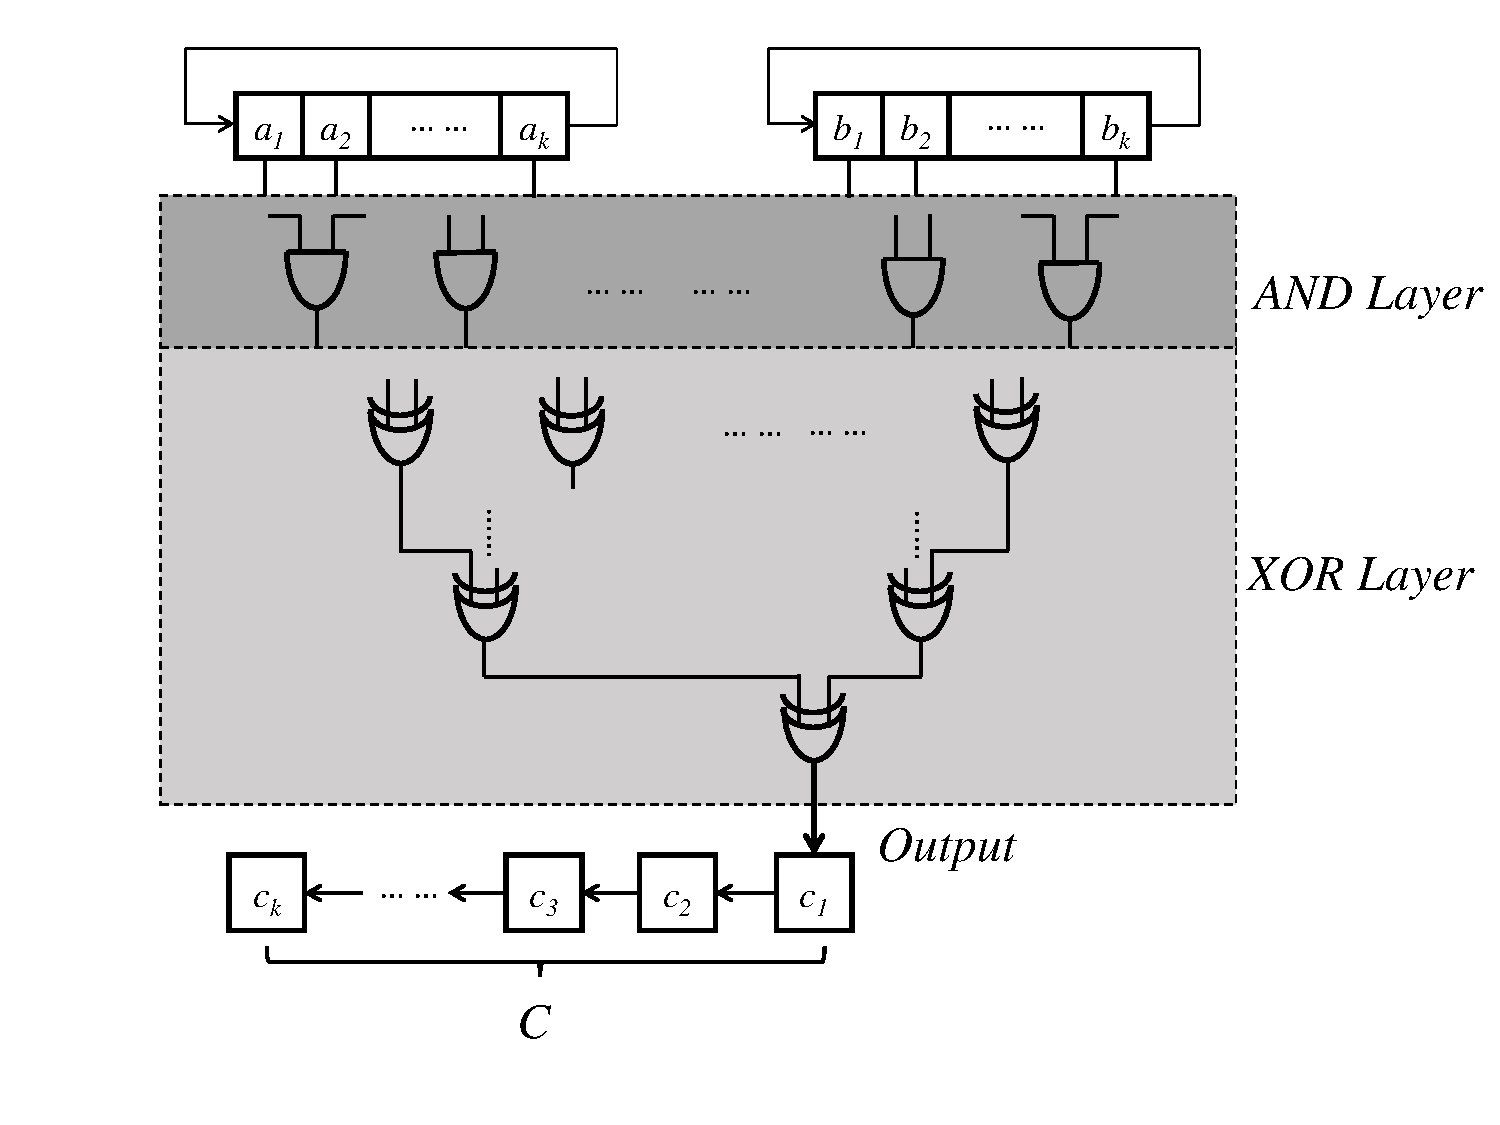
\includegraphics[width=\textwidth]{newfig/MasseyOmura.pdf}
\caption{A typical SMSO structure of Massey-Omura multiplier.}
\label{fig:MasseyOmura}}
\end{figure}

Figure \ref{fig:MasseyOmura} shows the basic architecture of a Massey-Omura multiplier. The operands
$A$ and $B$ are 2 arrays of flip-flops which allow 1-bit right-cyclic shift every clock cycle.
The logic gates in the boxes implements the matrix multiplication with $\lambda$-Matrix $M^{(0)}$, 
while each AND gate corresponds to term $a_ib_j$ and each XOR gate corresponds to addition $a_ib_j+a_{i'}b_{j'}$. 
The XOR layer has only 1 output, giving out 1 bit of product $C$ every clock cycle.

The behavior of Massey-Omura multiplier can be described as: pre-load operands $A,B$ and reset $C$ to 0, after 
executing for $k$ clock cycles, the data stored in flip-flop array $C$ is the product $A\times B$.
We note that there is only one output giving 1 bit of the product each clock cycle, which matches the 
definition of serial output to communication channel. Therefore this type of design is named as 
sequential multiplier with serial output (SMSO).
The SMSO architecture need $C_N$ AND gates and $C_N-1$ XOR gates, which equals to $2k-1$ AND gates and $2k-2$ XOR gates
if it is designed using ONB. In fact, the number of gates can be reduced if the multiplication is 
implemented using a conjugate of SMSO.

The gate-level logic boxes implement the following function:
\begin{equation}
\label{eqn:SMPOterms}
c_l = row_1(A\times M^{(l)}) \times B + row_2(A\times M^{(l)}) \times B + \cdots + row_{k}(A\times M^{(l)}) \times B
\end{equation}
It can be decomposed into $k$ terms. If we only compute one term for each $c_l,~0\leq l\leq k-1$ in one 
clock cycle, make $k$ outputs and add them up using shift register after $k$ clock cycles, 
it will generate the same result with SMSO. This kind of architecture is named as a 
sequential multiplier with parallel outputs (SMPO). The basic SMPO, as a conjugate of Massey-Omura multiplier,
was invented by Agnew {\it et al.} \cite{agnew1991implementation}.

\begin{figure}[H]
\centering{
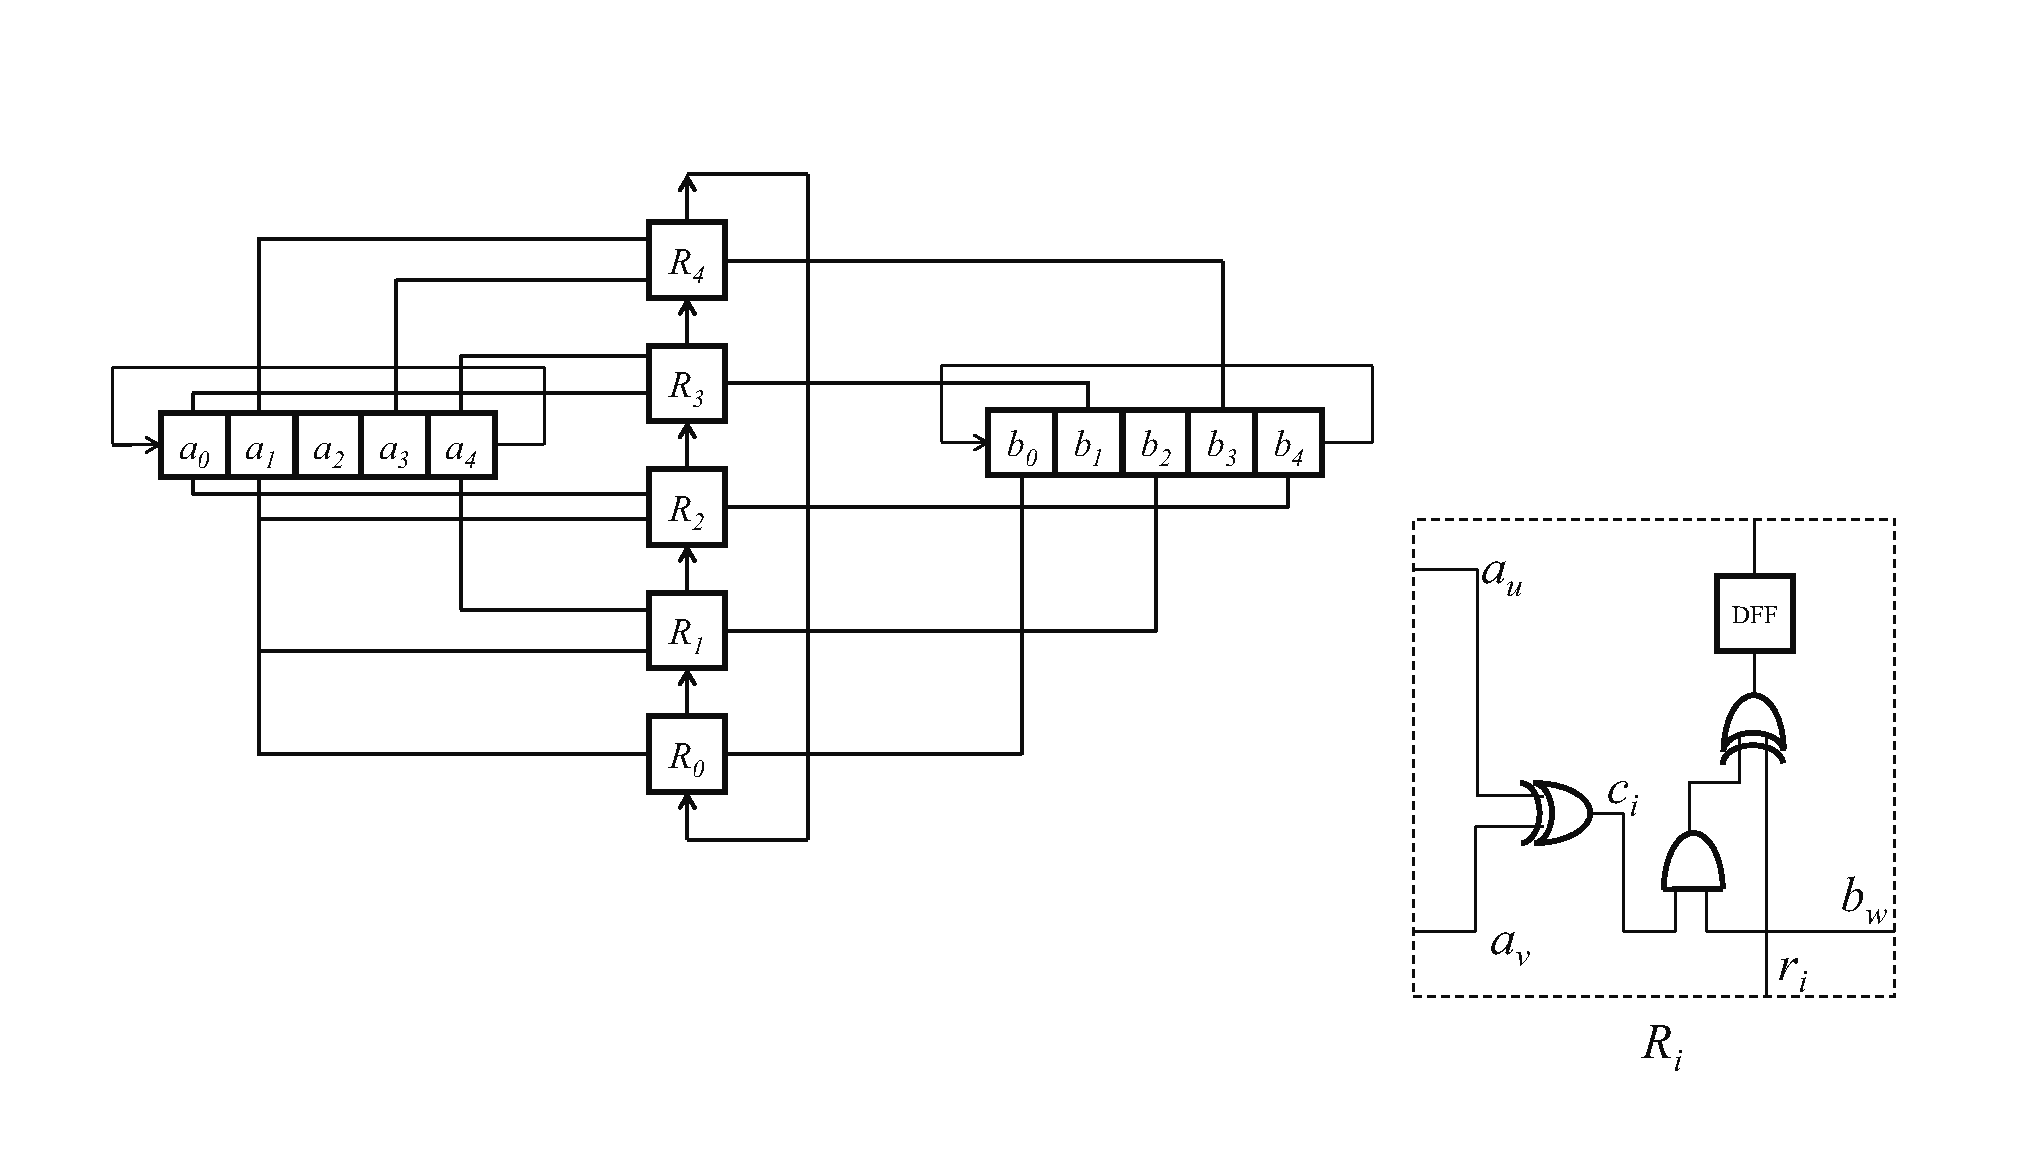
\includegraphics[width=\textwidth]{newfig/mySMPO.eps}
\caption{5-bit Agnew's SMPO. Index $i$ satisfies $0<i<4$, indices $u,v$ are determined by column \# of nonzero entries in $i$-th row of $\lambda$-Matrix $M^{(0)}$, {\it i.e.} if entry $M_{ij}^{(0)}$ is a nonzero entry, $u$ or $v$ equals to $i+j \pmod 5$. Index $w = 2i\pmod 5$.}
\label{fig:SMPO}}
\end{figure}

\begin{Example}[5-bit Agnew's SMPO]
Given GF $\mathbb F_{2^5}$ and primitive element $\alpha$ defined by irreducible polynomial 
$\alpha^5+\alpha^2+1=0$, normal element $\beta = \alpha^5$ constructs an ONB $\{\beta,\beta^2,\beta^4,\beta^8,\beta^{16}\}$.
The $0$-th $\lambda$-Matrix for this ONB is
\begin{equation*}
M^{(0)} = \left(\begin{array}{lcccr}
0 &1 &0 &0 &0 \\
1 &0 &0 &1 &0 \\
0 &0 &0 &1 &1 \\
0 &1 &1 &0 &0 \\
0 &0 &1 &0 &1
\end{array}\right)
\end{equation*}
Then a typical design of 5-bit Agnew's SMPO is depicted in Figure \ref{fig:SMPO}.

The operands part of this circuit is the same with Massey-Omura multiplier. The differences are on 
the matrix multiplication part, while it is implemented as separate logic blocks for 5 outputs,
and the 5 blocks are connected in a shift register fashion. By analyzing the detailed function of 
logic blocks, we can reveal the mechanism of Agnew's SMPO.

Suppose we implement $M^{(0)}$ as the logic block in SMSO. In the first clock cycle, the output is
\begin{equation}
\label{eqn:5bitSMPO_c0}
c_0 = a_1b_0+(a_0+a_3)b_1 + (a_3+a_4)b_2 + (a_1+a_2)b_3 + (a_2+a_4)b_4
\end{equation}
It is written in the form of Equation \ref{eqn:SMPOterms}. In next clock cycles we can obtain 
remaining bits of the product, which can be written in following general form polynomial:
\begin{align}
c_i =& b_ia_{i+1} + b_{i+1}(a_i + a_{i+3}) + b_{i+2}(a_{i+3} + a_{i+4}) \nonumber\\
&+ b_{i+3}(a_{i+1} + a_{i+2}) + b_{i+4}
(a_{i+2} + a_{i+4}),\ 0\leq i\leq 4 \nonumber
\end{align}
Note all index calculations are reduced modulo 5.

Now let us observe the behavior of 5-bit Agnew's SMPO. Initially all DFFs are reset to 0. 
In the first clock cycle,
signal sent to the flip-flop in block $R_0$ denotes function:
$$R_0^{(1)} = a_1b_0$$
It equals to the first term of Equation \ref{eqn:5bitSMPO_c0}. In the second clock cycle,
this signal is sent to block $R_1$ through wire $r_0$, and this block also receives data 
from operands (shifted by 1 bit), generating signal $a_u,a_v$ and $b_w$. Concretely,
signal sent to flip-flop in block $R_1$ is:
$$R_1^{(2)} = R_0^{(1)} + (a_0+a_3)b_1 = a_1b_0+(a_0+a_3)b_1$$
which forms first 2 terms of Equation \ref{eqn:5bitSMPO_c0}. Similarly, we track the signal 
on $R_2$ in third clock cycle, signal on $R_3$ in fourth clock cycle, finally we can get 
$$R_4^{(5)} = a_1b_0+(a_0+a_3)b_1 + (a_3+a_4)b_2 + (a_1+a_2)b_3 + (a_2+a_4)b_4$$
which equals to $c_0$ in Equation \ref{eqn:5bitSMPO_c0}.
After the fifth clock cycle ends, this signal can be detected on wire $r_0$. It shows that 
the result of $c_0$ is computed after 5 clock cycles and given on $r_0$.

If we track $R_1\to R_2\to R_3 \to \cdots \to R_0$, we can obtain $c_1$ respectively.
Thus we conclude that Agnew's SMPO functions the same with Massey-Omura multiplier.
\end{Example}

The design of Agnew's SMPO guarantees that there is only one AND gate in each $R_i$ block.
For ONB, adopting Agnew's SMPO will reduce the number of AND gates from $2k-1$ to $k$.

\subsection{Multiplier not based on the $\lambda$-Matrix}
Both Massey-Omura multiplier and Agnew's SMPO rely on the implementation of $\lambda$-Matrix,
which means that they will be identical if unrolled to full combinational circuits. 
After Agnew's work of parallelization, researchers proposed more designs of SMPO, 
some of them jump out of the box and are independent from $\lambda$-Matrix.
One competitive multiplier design of this type is invented by Reyhani-Masoleh and Hasan 
\cite{RHmulti}, which is therefore called RH-SMPO.

\begin{figure}[H]
\centering{
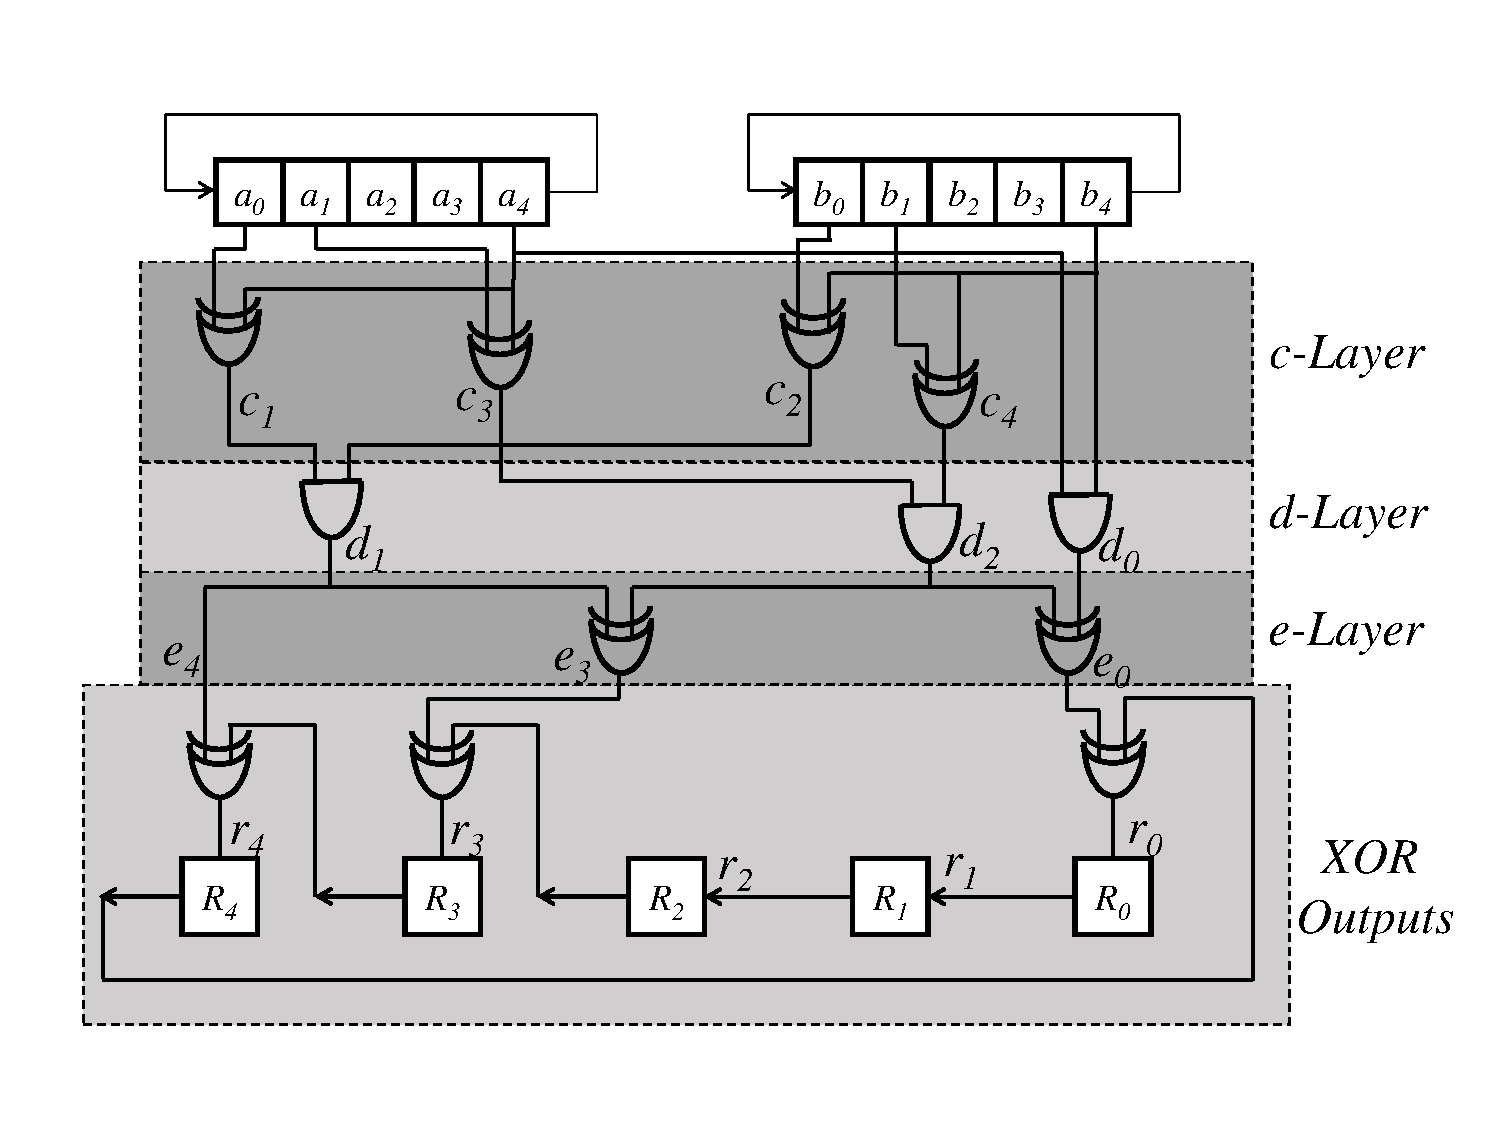
\includegraphics[width=\textwidth]{newfig/5bitRH.pdf}
\caption{A 5-bit RH-SMPO.}
\label{fig:5bitRH}}
\end{figure}

Figure \ref{fig:5bitRH} is a 5-bit RH-SMPO which is functionally equivalent to 5-bit Agnew's SMPO 
in Figure \ref{fig:SMPO}. A brief proof is as follows: 

\begin{Proof}
First, we define an auxiliary function for $i$-th bit 
\begin{equation}
\label{eqn:aux}
F_i(A,B) = a_ib_i\beta + \sum_{j=1}^v d_{i,j}\beta^{1+2^j}
\end{equation}
where $0\leq i\leq k-1, v = \lfloor k/2\rfloor, 1\leq j \leq v$.
The $d$-layer index $d_{i,j}$ is defined as
\begin{equation}
\label{eqn:auxDC}
d_{i,j} = c_{a,i} c_{b,i} = (a_i+a_{i+j})(b_i+b_{i+j}),~~1\leq j\leq v
\end{equation}
$i+j$ here is the result reduced modulo $k$. Note that there is a special boundary case when
$k$ is an even number ($v = \frac{k}{2}$):
$$d_{i,v} = (a_i+a_{i+v})b_i$$
With the auxiliary function, we can utilize following theorem (proof refers to \cite{RHmulti}):
\begin{Theorem}
Consider three elements $A,B$ and $R$ such that $R=A\times B$ over $\Fkk$. Then,
$$R=(((F_{k-1}^2+F_{k-2})^2+F_{k-3})^2+\cdots+F_1)^2+F_0$$
\end{Theorem}
where $F$ is as given in Equation \ref{eqn:aux}.
This form is called inductive sum of squares, and corresponds to the cyclic shifting on 
$R_i$ flip-flops. Concretely, the multiplier behavior is an implementation of 
following algorithm:

\begin{algorithm}[H]
\SetAlgoNoLine

 \KwIn{$A,B\in \Fkk$ given {\it w.r.t.} NB $N$}
 \KwOut{$R=A\times B$}
%%%%%%%%%%%%%%%%%%%%
  Initialize $A,B$ and aux var $X$ to 0\;
  \For { ($i=0$;   $i < k$; ++i ) }
  {
	$X \gets X^2+F_{k-1}(A,B)$ \CommentSty{/*use aux-func from Equation \ref{eqn:aux}*/\;}
	$A\gets A^2,~B\gets B^2$ \CommentSty{/*Right-cyclic shift $A$ and $B$*/\;}
  }
  $R\gets X$
\caption{NB Multiplication Algorithm in RH-SMPO \cite{RHmulti}}\label{alg:RHmulti}
\end{algorithm}

In this algorithm, we use a fixed auxiliary function $F_{k-1}$ inside the loop.
This is because of equation
$$F_{k-l} = F_{k-1}(A^{2^{l-1}},B^{2^{l-1}}),~~1\le l\le k$$
So using fixed $F_{k-1}$ and squaring $A^{2^i}$ every time inside the loop is equivalent to computing 
$F_{k-1},F_{k-2},\dots,F_0$ with fixed operands $A,B$.
\end{Proof}

To better understand the mechanism of RH-SMPO, we will use this 5-bit 
RH-SMPO as an example and introduce the details on how to design it.
\begin{Example}[Designing a 5-bit RH-SMPO]
From Equation \ref{eqn:aux} we can deploy AND gates in $d$-layer according to $d_{i,j}$,
and XOR gates in $c$-layer according to Equation \ref{eqn:auxDC}. Concretely, as Algorithm \ref{alg:RHmulti}
describes, we implement auxiliary function $F_{k-1}$ in the logic:
$$i = k-1 = 4;~~v=\lfloor 5/2 \rfloor = 2$$
\begin{equation}
\label{eqn:5bitRHaux}
F_{4}(A,B) = a_4b_4\beta+\sum_{j=1}^2 d_{4,j}\beta^{1+2^j} = d_0\beta+\sum_{j=1}^2 d_{4,j}\beta^{1+2^j}
\end{equation}
Consider indices $4+1=0\bmod 5,~4+2=1\bmod 5$, write down gates in $c$-layer and $d$-layer (besides $d_0$)
$$c_1 = a_0+a_4,~c_2 = b_0+b_4,~d_1=d_{4,1}= c_1c_2 = (a_4+a_0)(b_4+b_0)$$
$$c_3 = a_1+a_4,~c_4 = b_1+b_4,~d_2=d_{4,2}= c_3c_4 = (a_4+a_1)(b_4+b_1)$$
The difficult part of the whole design is to deploy XOR gates in $e$-layer. 
As the logic layer closest to the outputs $R_i$, $e$-layer actually finishes the implementation of 
$F_{k-1}(A,B)$. But it is not a simple addition; the reason is before bit-wise adding to $X^2$, it is necessary to 
turn the sum to NB form. In other words, theoretically we need $k$ XOR gates in $e$-layer, the output of 
$i$-th gate forms the coefficient of $\beta^{2^i}$.

In order to obtain information 
indicating interconnections between the $d$-layer and $e$-layer, we need to interpret $\beta^{1+2^j}$ 
to NB representation.
There is a concept called {\bf multiplication table} (M-table) which can assist this interpretation. It is defined as 
a $k\times k$ matrix $T$ over $\mathbb F_2$:
\begin{equation}
\label{eqn:multitable}
\begin{bmatrix}
\beta^{1+2^0} \\ \beta^{1+2^1} \\ \beta^{1+2^2} \\ \vdots \\ \beta^{1+2^{k-1}}
\end{bmatrix}
= \beta
\begin{bmatrix}
\beta \\ \beta^2 \\ \beta^4 \\ \vdots \\ \beta^{2^{k-1}}
\end{bmatrix}
=
\begin{bmatrix}
T_{0,0}      &   T_{0,1}        & \dots & T_{0,k-1}\\
T_{1,0}    &   T_{1,1}           & \dots & T_{1,k-1}\\
T_{2,0}    &   T_{2,1}           & \dots & T_{2,k-1}\\
\vdots & \vdots              & \ddots     & \vdots \\
T_{k-1,0}    &   T_{k-1,1}           & \dots & T_{k-1,k-1}
\end{bmatrix}
\begin{bmatrix}
\beta \\ \beta^2 \\ \beta^4 \\ \vdots \\ \beta^{2^{k-1}}
\end{bmatrix}
= {\bf T}
\begin{bmatrix}
\beta \\ \beta^2 \\ \beta^4 \\ \vdots \\ \beta^{2^{k-1}}
\end{bmatrix}
\end{equation}

It is a known fact that M-table $T$ can be converted from $\lambda$-Matrix $M$:
$$M_{i,j}^{(0)} = T_{j-i,-i}$$
with indices reduced modulo $k$ (proof given in Appendix \ref{append:ONB}). Thus we can write down the M-table of $\mathbb F_{2^5}$ with current NB $N$:

\begin{figure}[H]
\centering{
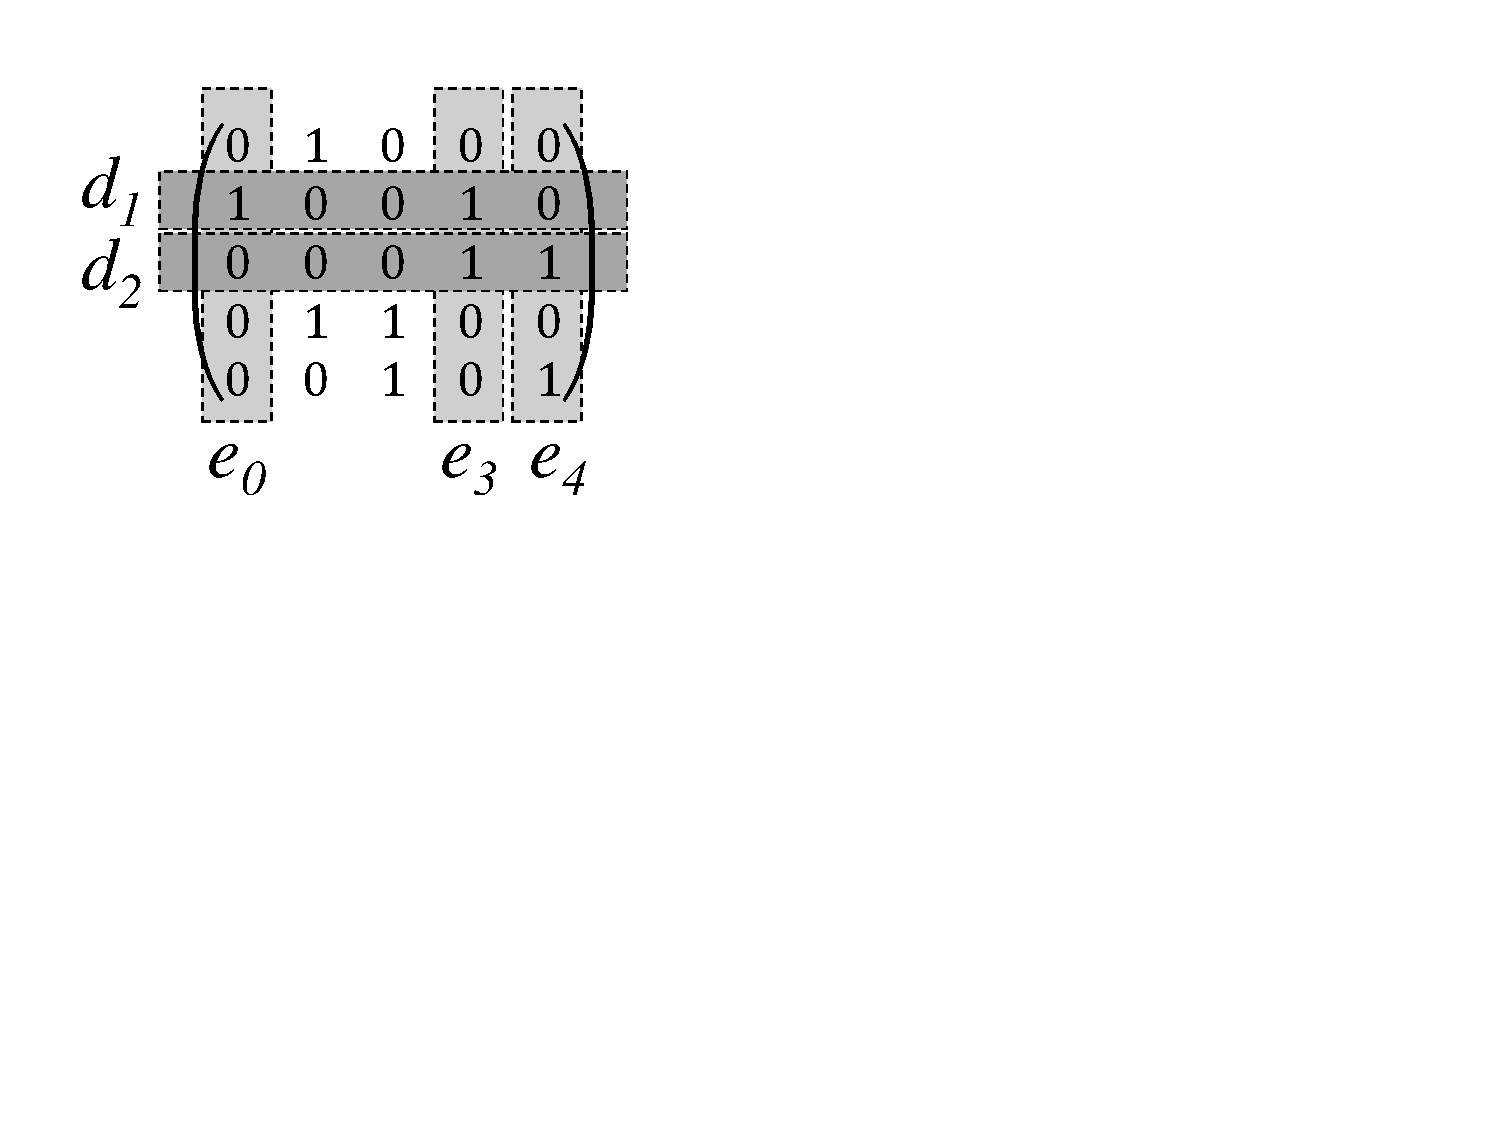
\includegraphics[width=3in]{newfig/multitable.pdf}
\caption{A $5\times 5$ multiplication table.}
\label{fig:multitable}}
\end{figure}

Note that we only use row 1 and row 2 from the M-table since range $1\leq j \leq 2$.
All nonzero entries in these 2 rows corresponds to the interconnections between $d$-layer and 
$e$-layer. For example, row 1 has two nonzero entries at column 0 and column 3, which corresponds to interconnections 
between $d_1$ and $e_0,e_3$. This conclusion comes from row 1 in Equation \ref{eqn:multitable}:
\begin{equation*}
\beta\cdot\beta^2 = 
\begin{bmatrix}
1 & 0 & 0 & 1 & 0
\end{bmatrix}
\begin{bmatrix}
\beta \\ \beta^2 \\ \beta^4 \\ \beta^8 \\ \beta^{16}
\end{bmatrix}
= \beta + \beta^{2^3}
\end{equation*}

Similarly, from row 2 of M-table we derive that $d_2$ has fanouts $e_3,e_4$:
\begin{equation*}
\beta\cdot\beta^{2^2} = 
\begin{bmatrix}
0 & 0 & 0 & 1 & 1
\end{bmatrix}
\begin{bmatrix}
\beta \\ \beta^2 \\ \beta^4 \\ \beta^8 \\ \beta^{16}
\end{bmatrix}
= \beta^{2^3} + \beta^{2^4}
\end{equation*}

Let us look back at Equation \ref{eqn:5bitRHaux}, we already dealt with the latter part.
The first term is always $d_0\beta$, which denotes $d_0$ should always be connected to $e_0(\beta)$.
After gathering all interconnection information, we can translate it to gate-level circuit implementation:
$$e_0 = d_0+d_1,~e_3=d_1+d_2,~e_4=d_2$$

Then the last mission is to implement the output $R_i$ layer. Assume $r_{i-1}$ is the output of 
$R_{i-1}$ in last clock cycle, we can connect using relation 
$$R_i = r_{i-1} + e_i$$
In this example, according to the M-table in Figure \ref{fig:multitable}, columns $e_1,e_2$
have only zeros in its intersection with row $d_1,d_2$. Thus gates for $e_1,e_2$ can be omitted.

This finishes the full design procedure for a 5-bit RH-SMPO.
\end{Example}

The area cost of RH-SMPO is even smaller than Agnew's SMPO. XOR gates corresponds to all nonzero entries 
in M-table, which is with the same number of nonzero entries in $\lambda$-Matrix ($C_N$). The number of AND gates 
equals to $v$ plus 1 (for gate $d_0$). When using ONB ($C_N = 2k-1$), the total number of gates 
is $2k+\lfloor \frac{k}{2}\rfloor$.

\section{Concluding Remarks}
In this chapter, we introduced basic concepts such as the definition of finite fields and the construction 
of finite fields. Moreover, we described a special kind of basis in finite field, and its 
application on Galois field hardware design. The sequential Galois field multipliers based on these 
principles are used as candidates for applying our functional verification approach in subsequent chapters.